\documentclass[12pt, a4paper, twoside]{scrartcl}
 %---- Allgemeine Layout Einstellungen ------------------------------------------

% Für Kopf und Fußzeilen, siehe auch KOMA-Skript Doku
\usepackage[komastyle]{scrpage2}
\pagestyle{scrheadings}
\setheadsepline{0.5pt}[\color{black}]


%Einstellungen für Figuren- und Tabellenbeschriftungen
\setkomafont{captionlabel}{\sffamily\bfseries}
\setcapindent{0em}


%---- Weitere Pakete -----------------------------------------------------------
% Die Pakete sind alle in der TeX Live Distribution enthalten. Wichtige Adressen
% www.ctan.org, www.dante.de

% Sprachunterstützung
\usepackage[ngerman]{babel}

% Benutzung von Umlauten direkt im Text
% entweder "latin1" oder "utf8"
\usepackage[utf8]{inputenc}

% Pakete mit Mathesymbolen und zur Beseitigung von Schwächen der Mathe-Umgebung
\usepackage{latexsym,exscale,stmaryrd,amssymb,amsmath}

% Weitere Symbole
\usepackage[nointegrals]{wasysym}
\usepackage{eurosym}

% Anderes Literaturverzeichnisformat
%\usepackage[square,sort&compress]{natbib}

% Für Farbe
\usepackage{color}

% Zur Graphikausgabe
%Beipiel: \includegraphics[width=\textwidth]{grafik.png}
\usepackage{graphicx}

% Text umfließt Graphiken und Tabellen
% Beispiel:
% \begin{wrapfigure}[Zeilenanzahl]{"l" oder "r"}{breite}
%   \centering
%   \includegraphics[width=...]{grafik}
%   \caption{Beschriftung} 
%   \label{fig:grafik}
% \end{wrapfigure}
\usepackage{wrapfig}

% Mehrere Abbildungen nebeneinander
% Beispiel:
% \begin{figure}[htb]
%   \centering
%   \subfigure[Beschriftung 1\label{fig:label1}]
%   {\includegraphics[width=0.49\textwidth]{grafik1}}
%   \hfill
%   \subfigure[Beschriftung 2\label{fig:label2}]
%   {\includegraphics[width=0.49\textwidth]{grafik2}}
%   \caption{Beschriftung allgemein}
%   \label{fig:label-gesamt}
% \end{figure}
\usepackage{subfigure}

% Caption neben Abbildung
% Beispiel:
% \sidecaptionvpos{figure}{"c" oder "t" oder "b"}
% \begin{SCfigure}[rel. Breite (normalerweise = 1)][hbt]
%   \centering
%   \includegraphics[width=0.5\textwidth]{grafik.png}
%   \caption{Beschreibung}
%   \label{fig:}
% \end{SCfigure}
\usepackage{sidecap}
\usepackage{float}

% Befehl für "Entspricht"-Zeichen
\newcommand{\corresponds}{\ensuremath{\mathrel{\widehat{=}}}}
\newcommand{\folgt}{\ensuremath{\mathrel{\Rightarrow}}}
\newcommand{\equals}{\ensuremath{\mathrel{\Leftrightarrow}}}
\newcommand{\degree}{\ensuremath{\mathrel{^{\circ}}}}

\newcommand{\nn}{\nonumber}
\newcommand{\tn}[1]{\textnormal{#1}}
\newcommand{\D}{\ensuremath{\mathrel{\rm d}}}

\newcommand{\const}{\tn{const}}

\newcommand{\meter}{\ensuremath{\mathrel{\tn m}}}
\newcommand{\kilogramm}{\ensuremath{\mathrel{\tn{kg}}}}
\newcommand{\second}{\ensuremath{\mathrel{\tn s}}}
\newcommand{\sekunde}{\second}

\newcommand{\volt}{\ensuremath{\mathrel{\tn V}}}
\newcommand{\pascal}{\ensuremath{\mathrel{\tn{Pa}}}}
\newcommand{\coulomb}{\ensuremath{\mathrel{\tn C}}}
\newcommand{\newton}{\ensuremath{\mathrel{\tn N}}}
\newcommand{\liter}{\ensuremath{\mathrel{\tn l}}}
\newcommand{\celsius}{\ensuremath{\mathrel{\tn C}}}
\newcommand{\fahrenheit}{\ensuremath{\mathrel{\tn F}}}
\newcommand{\joule}{\ensuremath{\mathrel{\tn J}}}
\newcommand{\kelvin}{\ensuremath{\mathrel{\tn K}}}
\newcommand{\mol}{\ensuremath{\mathrel{\tn{mol}}}}
\newcommand{\gramm}{\ensuremath{\mathrel{\tn{g}}}}

\newcommand{\kilo}{\ensuremath{\mathrel{\tn k}}}
\newcommand{\hecto}{\ensuremath{\mathrel{\tn h}}}

\newcommand{\centi}{\ensuremath{\mathrel{ \tn c}}}
\newcommand{\milli}{\ensuremath{\mathrel{ \tn m}}}
\newcommand{\micro}{\ensuremath{\mathrel{ \tn\mu }}}



%\newcommand{}{\ensuremath{\mathrel{  }}}
%\newcommand{}{\ensuremath{\mathrel{  }}}
%\newcommand{}{\ensuremath{\mathrel{  }}}


\newcommand{\person}[1]{\textsc{#1}}

 \begin{document}
 %Titelseite
\begin{titlepage}
\centering
\textsc{\Large Anfängerpraktikum der Fakultät für
  Physik,\\[1.5ex] Universität Göttingen}

\vspace*{4.2cm}

\rule{\textwidth}{1pt}\\[0.5cm]
{\huge \bfseries
  Spezifische Wärme der Luft und Gasthermometer}\\[0.5cm]
\rule{\textwidth}{1pt}

\vspace*{3.5cm}

\begin{Large}
\begin{tabular}{ll}
Praktikanten: &  Silke Andrea Teepe\\
& Marcel Kramer\\
E-Mail: & \\
Betreuer: & Alexander Schmelev\\
\end{tabular}
\end{Large}

\vspace*{0.8cm}

\begin{Large}
\fbox{
  \begin{minipage}[t][2.5cm][t]{6cm} 
    Testat:
  \end{minipage}
}
\end{Large}

\end{titlepage}
\cleardoublepage
\tableofcontents
\cleardoublepage
\setcounter{page}{1}

\section{Einleitung}


\section{Theorie}
\label{sec:theorie}
\subsection{\person{Van-der-Waals}-Gleichung}
Für ideale Gase gilt die Zustandsgleichung $p\cdot V = n\cdot R\cdot T$.
Doch für reale Gase kann diese Gleichung nicht gelten. \\
Zum einen hat ein reales Gas bei $0\kelvin$ im Gegensatz zum idealen Gas immernoch ein \textit{Eigenvolumen}, da die Gasmoleküle nicht punktförmig sind.
Dieses Eigenvolumen, das offensichtlich proportional zur Teilchenanzahl ist, muss folglich vom Gesammtvolumen abgezogen werden, also $V \rightarrow V-b\cdot n$ mit der \textit{Eigenvolumenkonstante} $b$.
\\
Zum anderen wirken Dipol-Dipol- und \person{Van-der-Waals}-Kräfte zwischen den Teilchen.
Wie in Versuch 5 beschrieben, sind diese Kräfte proportional zur Teilchenzahl an der Oberfläche, da sich die Kräfte im Inneren aufheben, und proportional zum mittleren Abstand der Teilchen.
Da sowohl die Teilchenanzahl an der Oberfläche, als auch der mittlere Teilchenabstand proportional zur Teilchendichte $n/V$ ist, ist der Druck $p$ in einem realen Gas um den \textit{Binnendruck} $a\cdot \frac{n^2}{V^2}$ größer, also $p \rightarrow p + a\cdot \frac{n^2}{V^2}$ mit der \textit{Binnendruckkonstanten} $a$.
\\
Unter Einbeziehung dieser Korrekturterme ergibt sich die \person{Van-der-Waals}-Gleichung
\begin{align}
 \left(p+a\cdot \frac{n^2}{V^2}\right) \cdot \left(V-b\cdot n\right) = n\cdot R\cdot T \label{VdW_Gleichung} \\
\equals 
 p = \frac{n\cdot R\cdot T}{V-b\cdot n}-a\cdot \frac{n^2}{V^2}\nn
\end{align}
\begin{figure}
 \centering
 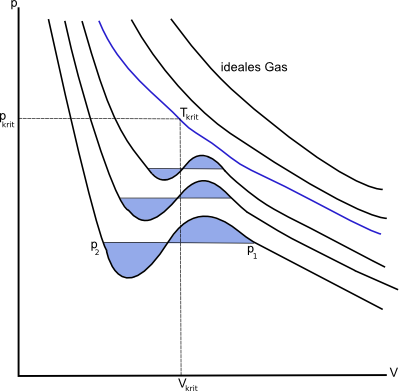
\includegraphics[scale=0.5]{maxwell.png}
 \caption{Isothermen der \person{Van-der-Waals}-Gleichung mit \person{Maxwell}-Geraden\protect\footnotemark\label{fig:maxwell}}
\end{figure}
\footnotetext{https://lp.uni-goettingen.de/get/text/655\;\;Abb. 732}

\subsection{\person{Maxwell}-Geraden}
Wie man in der Abbildung \ref{fig:maxwell} erkennen kann, haben die Isothermen der \person{Van-der-Waals}-Gleichung für Temperaturen unter $T_k$ ein Maximum und ein Minimum.
Dieser Bereich verletzt den zweiten Hauptsatz der Thermodynamik, denn wenn bei isothermer Expansion der Druck steigt, müssten bei steigendem Volumen mehr Teilchen auf eine konstante Fläche treffen, also müsste die Teilchendichte am Rand steigen und somit in der Mitte sinken.
Damit würde die Entropie sinken, was ein wiederspruch zum 2. Hauptsatz ist.
\\
Um dieses Problem zu lösen, werden die \person{Maxwell}-Geraden als isobare Verbindungsstücke so eingefügt, dass die Flächen zwischen der Isothermen der \person{Van-der-Waals}-Gleichung und der \person{Maxwell}-Geraden oberhalb und unterhalb dieser Geraden gleich groß sind (siehe Abbildung \ref{fig:maxwell}).
In diesem Bereich der Isothermen findet der Übergang von flüssig nach gasförmig statt.
\\
Für hohere Temperaturen wird die \person{Maxwell}-Gerade immer kleiner bis bei der kritischen Temperatur $T_k$ ein Sattelpunkt anstatt der Extrema vorliegt und es folglich keine \person{Maxwell}-Gerade mehr gibt.
Damit findet auch kein Aggregatszustandswechsel für Temperaturen über $T_k$ mehr statt.
Da ein Sattelpunkt vorliegt folgt aus der \person{Van-der-Waals}-Gleichung
\begin{align}
 T_k = \frac{8}{27}\cdot \frac{a}{R\cdot b}
\end{align}
und damit
\begin{align}
 V_k &= 3\cdot b \tn{\;\; und}\\
 p_k &= \frac{1}{27}\cdot \frac{a}{b^2}
\end{align}


\subsection{\person{Clausius-Clapeyron} Gleichung}
Wenn man ein $\mol$ einer Flüssigkeit in ein Gefäß mit einem größeren Volumen als $V_{fl}$ füllt, werden manche Moleküle verdampfen und es bildet sich eine Gasmenge über der Flüssigkeit mit dem Druck $p_s$.
Da zum austreten aus der Flüssigkeit Energie aufgewentet werden muss, kühlt sich die Flüssigkeit bzw. es muss eine Energiemenge $\Lambda_V$ hinzugefügt werden um die Temperatur konstant zu halten.
\\
Um diese Energiemenge für ein zu bestimmen betrachte man folgenden \person{Carnot}-Prozess: \\
\begin{itemize}
 \item $1\rightarrow 2$: isobare und isotherme Verdampfung von $V_1=V_{fl}$ bis $V_2=V_D$ bei $T_1=T+\tn{d}T$ und $p_1=p_s+\tn{d}p_s$, also eine \person{Maxwell}-Gerade 
 \item $2\rightarrow 3$: adiabatisch infinitesimal auf $T_2=T$ und $p_2=p_s$ reduziert und kein Aggregatszustandswechsel
 \item $3\rightarrow 4$: isobare und isotherme Konsensierung von $V_2=V_D$ bis $V_1=V_{fl}$ bei $T_2=T$ und $p_2=p_s$, also eine \person{Maxwell}-Gerade
 \item $4\rightarrow 1$: adiabatisch infinitesimal auf $T_1=T+\tn{d}T$ und $p_1=p_s+\tn{d}p_s$ erhöht und kein Aggregatszustandswechsel
\end{itemize}
Die verrichtete Arbeit ist somit
\begin{align}
 \Delta W_1 &= \left(p_s+\tn{d}p_s\right)\cdot \left(V_{fl}-V_D\right)  \tn{\;\; von } 1\rightarrow 2 \nn\\
 \Delta W_2 &= p_s\cdot \left(V_D-V_{fl}\right) \tn{\;\; von } 3\rightarrow 4 \nn\\
 \folgt \Delta W &= \Delta W_1 +\Delta W_2 = \tn{d}p_s\cdot \left(V_{fl}-V_D\right)
\end{align}
Da es sich um einen \person{Carnot}-Prozess handelt gilt für den Wirkungsgrad
\begin{align}
 \eta = -\frac{\Delta W}{\Delta Q} = \frac{T_{warm}-T_{kalt}}{T_{warm}} = \frac{T+\tn{d}T-T}{T+\tn{d}T} = \frac{\tn{d}T}{T+\tn{d}T} \approx \frac{\tn{d}T}{T} \nn
\end{align}
wobei $\Delta Q = \Lambda_V$ die hinzugefügte Energie ist. Es gilt also die \person{Clausius-Clapeyron} Gleichung
\begin{align}
\Lambda_V &= -\tn{d}p_s\cdot \left(V_{fl}-V_D\right)\cdot\frac{T}{\tn{d}T} \nn\\
          &= T\cdot \frac{\tn{d}p_s}{\tn{d}T}\cdot \left(V_D-V_{fl}\right)
\end{align}
Aus der idealen Gasgleichung folg für $n = 1\mol$
\begin{align}
 p_s\cdot V_D \approx R\cdot T\cdot\nn
\end{align}
Wenn der Außendruck nicht zu hoch ist gilt im Allgemeinen $V_D \gg V_{fl}$. Durch einsetzen erhält man 
\begin{align}
 \Lambda_V &= T\cdot \frac{\tn{d}p_s}{\tn{d}T}\cdot \frac{R\cdot T}{p_s} \nn\\
 \equals \frac{\Lambda_V \cdot \tn{d}T}{R\cdot T^2}&= \frac{\tn{d}p_s}{p_s} \nn
\end{align}
durch beidseitiges Integrieren erhält man
\begin{align}
  ln\left(p_s\right) = -\frac{\Lambda_V}{R\cdot T} + \const
\end{align}
mit der Randbedingung $p_s(T_0) = p_0$ folgt die Dampfdruckformel
\begin{align}
 p_s = p_0 \cdot \exp\left[\frac{\Lambda_V}{R}\cdot \left(\frac{1}{T_0}-\frac{1}{T}\right)\right]
\end{align}

%\subsection{Widerstandsthermometer}

\section{Durchführung}
\label{sec:durchfuehrung}

Zur Messung des Dampfdrucks von Wasser ist ein abgeschlossener Kolben zum Teil mit Wasser gefüllt. Dieser Kolben ist auf einer Heizplatte platziert, wodurch dieser erhitzt werden kann. Die Temperatur kann an dem angeschlossenen Pt1000 Widerstandsthermometer abgelesen werden. Der Druck an einem verbundenen Manometer. Aufgrund der hohen Temperatur die während des Experiments erreicht wird gehört aus Sicherheitsgründen auch eine Plexiglas-Schutzscheibe zum Versuchsaufbau. Der beschriebene Aufbau ist auch in Abbildung \ref{img:aufbau} zu sehen.\\


Ziel des Experimentes ist es, die Temperatur in Abhängigkeit des Drucks zu messen. Dazu schaltet man zunächst die Heizplatte ein und notiert dann die entsprechenden Werte von den beiden Messgeräten. Es empfiehlt sich dabei eine Skaleneinteilung von 1-2 bar zu wählen. Sobald entweder $45$ bar oder $1900\,\Omega$ $(240\degree\celsius)$ erreicht sind ist die Heizplatte auszuschalten und die Messung für das Abkühlen zu wiederholen.

\begin{figure} [h]
\centering
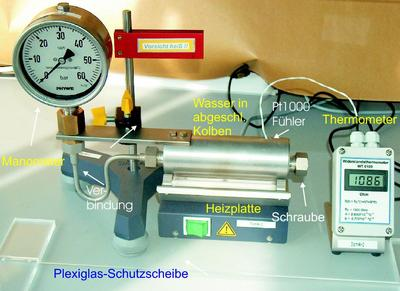
\includegraphics[scale=0.8]{aufbau.jpg}
\caption{\label{img:aufbau}Aufbau des Experiments\protect\footnotemark}
\end{figure}
\footnotetext{https://lp.uni-goettingen.de/get/text/3644}



\section{Auswertung}
\label{sec:auswertung}

\section{Diskussion}
\label{sec:diskussion}

\section*{Literatur}


\end{document}
